% LaTeX file for a 1 page document
\documentclass[11pt]{article}
\usepackage{amsmath}
\usepackage{amssymb}
\usepackage{amsthm}
%\usepackage{physymb}
\usepackage{graphicx}
%\usepackage{wrapfig}
\bibliographystyle{plain}
\usepackage{tikz}
\usepackage{natbib}
\usetikzlibrary{calc,patterns,decorations.pathmorphing,decorations.markings}

\title{Physics Behind the Simulation: A CS296 Report by Group 07}
\author{Ranveer Aggarwal (120050020) \\ ranveeraggarwal@gmail.com \\ Devdeep Ray (120050007) \\ devdeep.ray1994@iitb.ac.in\\ Sasibhushan Rallabandi (120050056) \\ sasiralla@iitb.ac.in}
\date{January 24, 2014}

\begin{document}
\maketitle

\section{Introduction}
This report aims at explaining modifications and the physics behind those modifications we performed in the base code of the \textbf{Rube Goldberg simulation} that was given to us in intially.

The simulation uses Box2D. Box2D is a free open source 2-dimensional physics simulator engine written in C++. \cite{b2d} The given base code had a simulation of the Rube Goldberg machine, which is basically a contraption where laws of physics are used to simulate different objects on the screen. The task assigned was to make the given simulation more interesting by adding more objects to it. So we added a few planks, a pendulum rod and a ball, increasing the complexity of the simulation.

The next section of this report is aimed at explaining the physics behind the objects that we added -- in plain English and also mathematically.
\pagebreak

\section{Physics behind the simulation}

\setlength\fboxsep{2pt}
\setlength\fboxrule{1pt}
\fbox{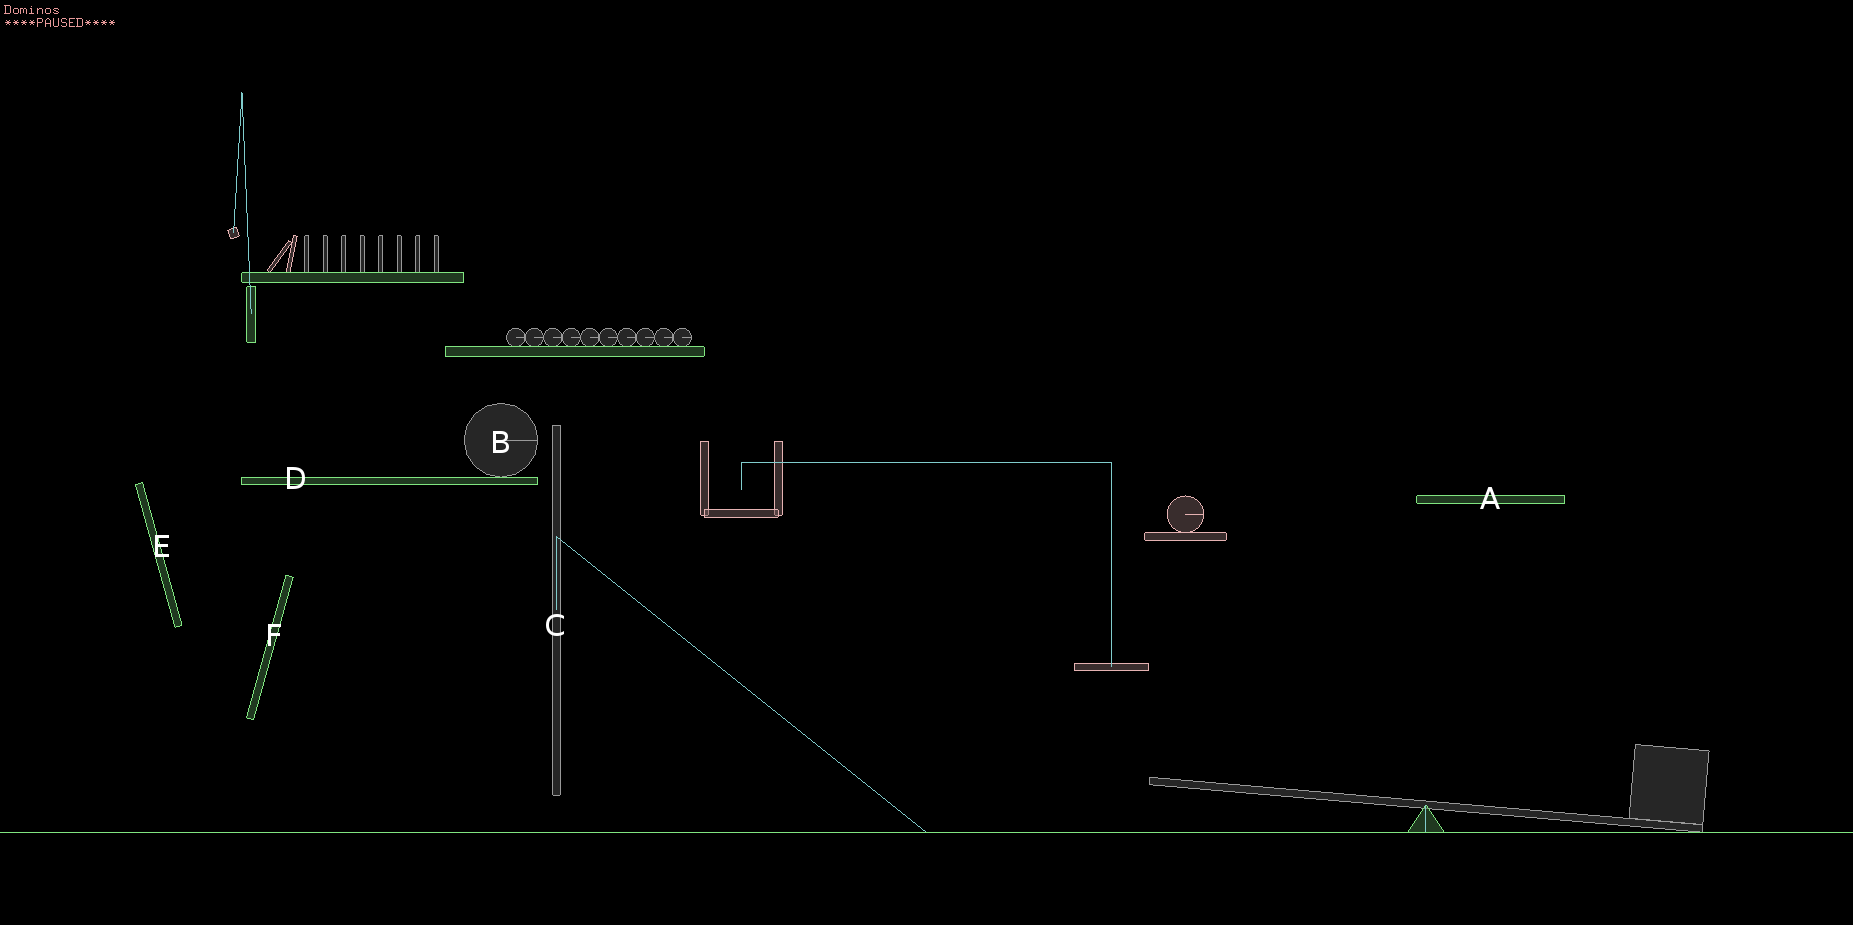
\includegraphics[scale=0.2]{./img/8.png}}
\\
\\
Following are the new additions in the original setup:
\begin{itemize}
\item[A] An immovable plank
\item[B] A ball of radius twice the original one
\item[C] A pendulum rod
\item[D-F] Immovable planks to make way for B
\end{itemize}
All these are explicitly explained in the following subsections.

\pagebreak

\subsection{Immovable plank A}
\setlength\fboxsep{2pt}
\setlength\fboxrule{1pt}
\fbox{
\includegraphics[scale=0.5]{./img/5.png}}
\\

Plank A  is the plank on which the box lands after completing it's projectile trajectory. The following equations hold \cite{hcv} (for the centre of mass of the box):
\begin{align}
\frac{d^2 y}{dt^2} = g &&\mbox{(The downwards acceleration)}&
\\
\frac{dx}{dt} = ucos\theta &&\mbox{(Horizontal Velocity)}&
\\
y = xtan\theta - \frac{g}{(2u^2 cos^2 \theta)}x^2 &&\mbox{(Equation of Trajectory)}&
\end{align}
where,\\
$g$ is the downward acceleration in $m/s^2$,\\
$\theta$ is the angle that the trajectory makes with the horizontal initially and\\
$u$ is the initial velocity in $m/s$.

After the completing of motion, this is how it looks: \\
\\
\setlength\fboxsep{2pt}
\setlength\fboxrule{1pt}
\fbox{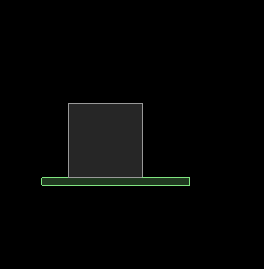
\includegraphics[scale=0.5]{./img/6.png}}
\\

and it stays there.

\pagebreak

\subsection{The Ball B}
The ball recieves an impulse from the pendulum rod C and it starts to slide down plank D. Friction comes into action and reduces the velocity, increasing the angular velocity from $0$ to $\omega '$ till it starts rolling. When the plank ends, it falls off the edge and slids onto planks E and F. \cite{halliday} After several collisions with the two planks, it goes through the gap between the ends of the two plank and goes out of the frame, colliding with the ground.\\
\\
\setlength\fboxsep{2pt}
\setlength\fboxrule{1pt}
\fbox{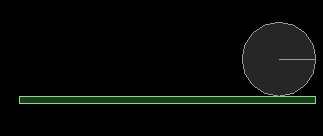
\includegraphics[scale=0.5]{./img/1.png}}
\\

Impulse it recieves from C is given by:
\begin{align}
J_B = m_B v_B
\end{align}
where,\\
$J_B$ is the impulse it recieves from rod C in $Kg m/s^2$,\\
$m_B$ is the mass of the ball in $Kg$ and\\
$v_B$ is the linear velocity in $m/s$.\\

This gives it a linear velocity $v_B = \frac{J_B}{m_B}$. Angular momentum about the contact point of the plank and the sphere is conserved. Hence
\begin{align}
m_B v_B r = m_B v'r + I\omega '
\\
v' = r\omega ' &&\mbox{(Pure rolling)}&
\end{align}
where,\\
$v'$ is the velocity after the ball attains pure rolling in $m/s$,\\
$r$ is the radius of the ball in $m$,\\
$I$ is the moment of inertia for the ball,\\
$\omega '$ is the angular velocity after the ball attains pure rolling and\\
the other symbols have the usual meanings.\\

We know that $I$ for a sphere is $\frac{2mr^2}{5}$.
Solving the above equations, we get:
\begin{align}
\omega ' = \frac{5v}{7r}
\end{align}

\pagebreak

After falling off the edge of D, it lands in between E and F, where it goes several collisions with coefficient of restitution, $e = 0.8$. \cite{halliday}
\begin{align}
\hat{v}_{\perp} ' = \hat{v}_{\perp}e
\\
\hat{v}_{\parallel} ' = \hat{v}_{\parallel}
\end{align}
where,\\
$\hat{v}_{\perp} '$ and $\hat{v}_{\parallel} '$ are the final velocities,\\
$\hat{v}_{\perp}$ and $\hat{v}_{\parallel}$ are the initial velocities and\\
$e$ is the coefficient of restitution.
\\
\\
\setlength\fboxsep{2pt}
\setlength\fboxrule{1pt}
\fbox{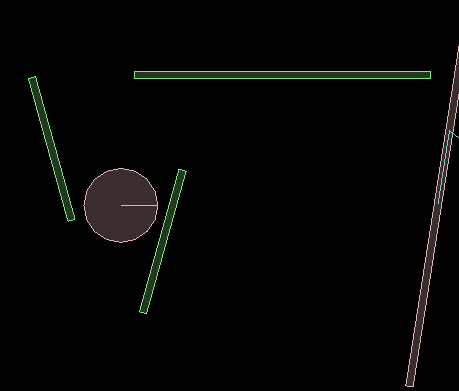
\includegraphics[scale=0.5]{./img/7.png}}
\\

Then, it collides with the ground, with it's height decreasing on each \\ collision.

\pagebreak

\subsection{Pendulum Rod}

\setlength\fboxsep{2pt}
\setlength\fboxrule{1pt}
\fbox{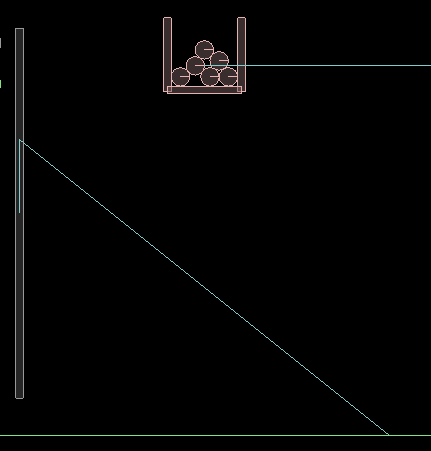
\includegraphics[scale=0.5]{./img/4.png}}
\\

The rod shown in the above picture, pivoted at the point where the blue line intersects, is free to rotate and works like a pendulum. The original ball strikes the lower end of the rod and gives it an impulse, due to which it starts oscillating on it's pivot. Then, it is during this motion that the upper end strikes the new ball which sets it into motion.

The total angular momentum of the ball+rod system is conserved because there is no external torque acting about the pivot. So, the following equation holds:

\begin{align}
mv_i x = I\omega_o + mv_f x
\end{align}
where,\\
$m$ is the mass of the ball B in $Kg$,\\
$v_i$ is the initial and $v_f$ is the final velocity in $m/s$,\\
$x$ is the distance of the pivot from the rod's ground-end and\\
$I$ is the moment of inertia of the rod about the pivot, derivable through the parallel axes theorem.

\pagebreak

\section{Conclusion}
Hence, we explained the physics behind three new objects added to the initial contraption. We used pretty basic laws, assuming ideal conditions in all the cases. The principles of impulse, angular momentum, pure rolling, collision were widely demonstrated. The coefficients of restitution were varied to get an interesting overall simulation. 

\bibliography{report}

\end{document}
}
